\begin{chapter}{Introduction}
\label{ch:introduction}
In this chapter we give a short introduction to the underlying mathematical and physical ideas.
This work extends the work of \cite{FGL_semiclassical_dynamics} to the case of the Morse function as an example of an anharmonic yet still analytically solvable potential.\\


\section{The time-dependent Schrödinger equation} % (fold)
\label{sec:The time-dependent Schroedinger equation}
The time evolution of a wave function $\ket{\psi}$ is governed by the following partial differential equation
\begin{equation}
    i\hbar\pdiff{}{t}\ket{\psi}=H\ket{\psi}
\end{equation}


% section The time-dependent Schroedinger equation (end)

\section{The Morse Potential} % (fold)
\label{sec:morse_potential}
The Morse potential was first introduced by Philipp M. Morse \cite{PMMorse} modelling the potential energy of a diatomic molecule and has the following form
\begin{equation}
    M(x)=V_0(e^{-2\beta(x-x_0)}-2e^{-\beta(x-x_0)})
\end{equation}
In contrast to the harmonic oscillator it accounts for the anharmonicity of molecular bonds and also models the breaking of a bond which leads to a finite
number of discrete bound states transitioning into a continuum of unbound Morse states.\\

The parameter $V_0$ corresponds to the maximal depth of the potential well. The subtraction of the ground state energy yields
the dissociation energy necessary to break the bond. The parameter $x_0$ determines the position of the potential minimum and hence the equilibrium bond
distance of two atoms. Finally, the parameter $\beta$ roughly corresponds to the width of the well.  \\



\begin{figure}[h!]
    \centering
     \subfloat[][]{
	\label{fig:MorsePlot7_08_3}
	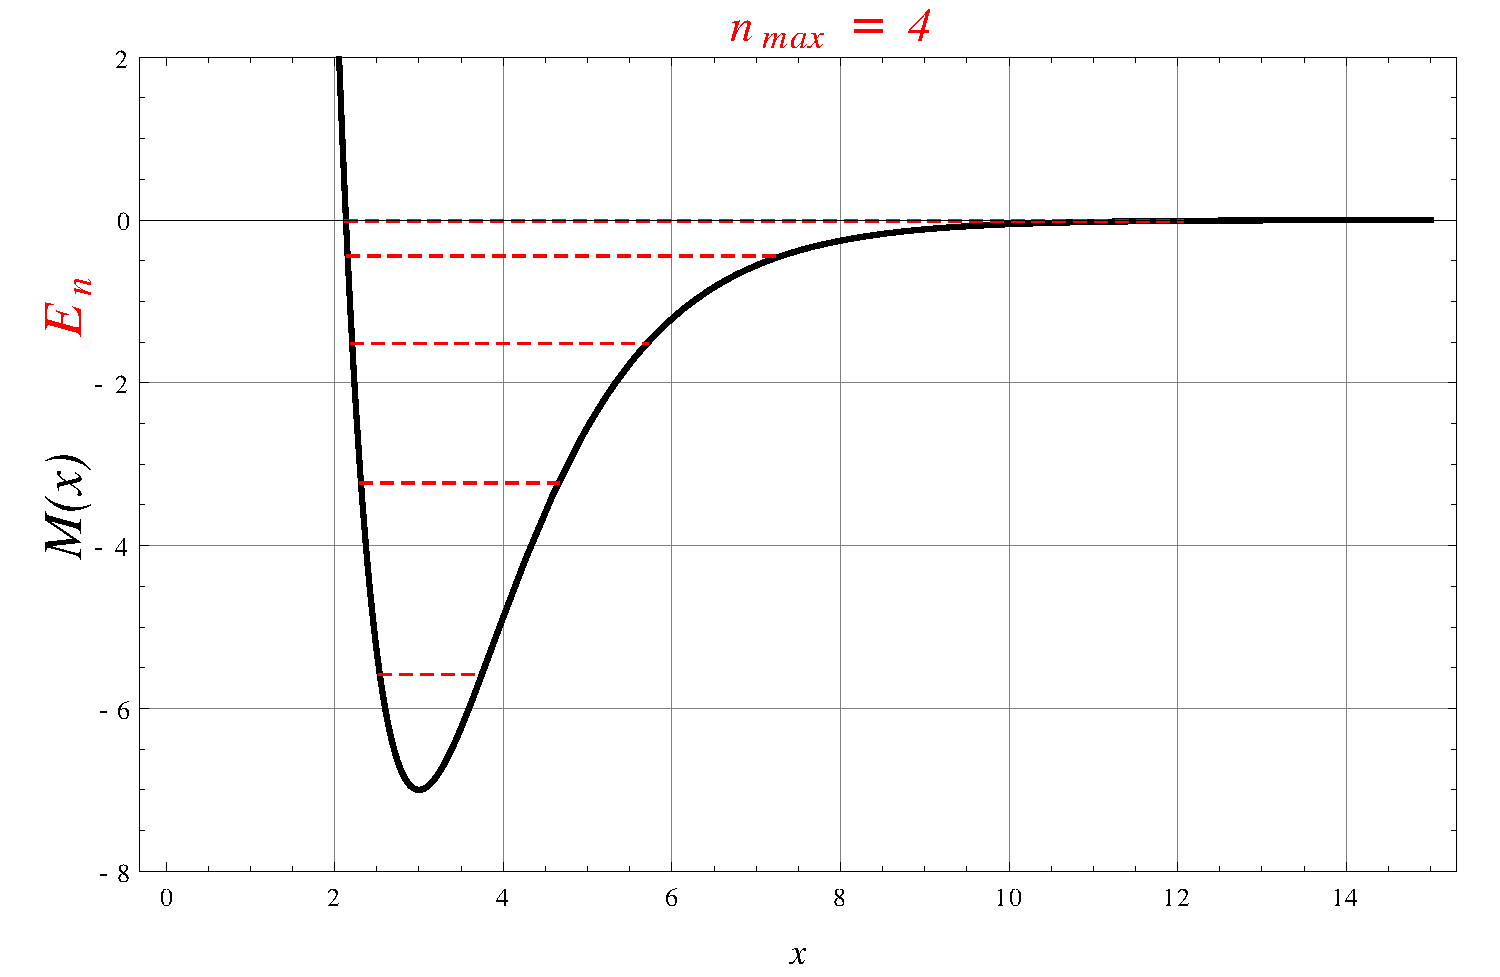
\includegraphics[width=0.5\linewidth]{./figures/MorsePlots/Morse7_08_3.pdf}
    }
    \subfloat[][]{
	\label{fig:MorsePlot5_05_3}
	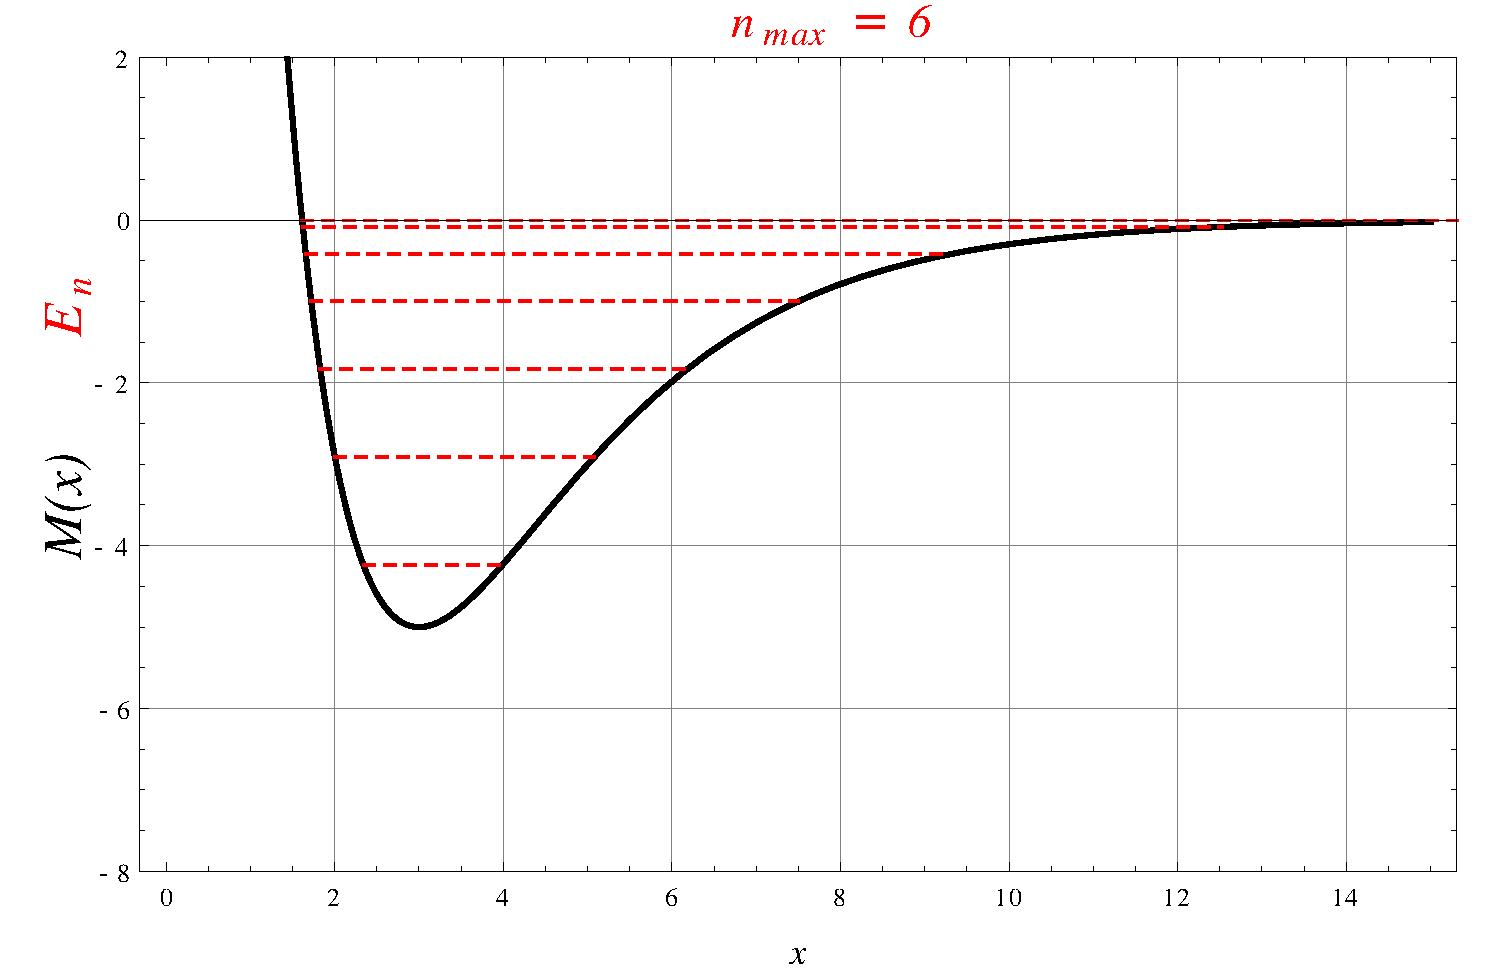
\includegraphics[width=0.5\linewidth]{./figures/MorsePlots/Morse5_05_3.pdf}
    }\\
    \subfloat[][]{
	\label{fig:MorsePlot7_03_3}
	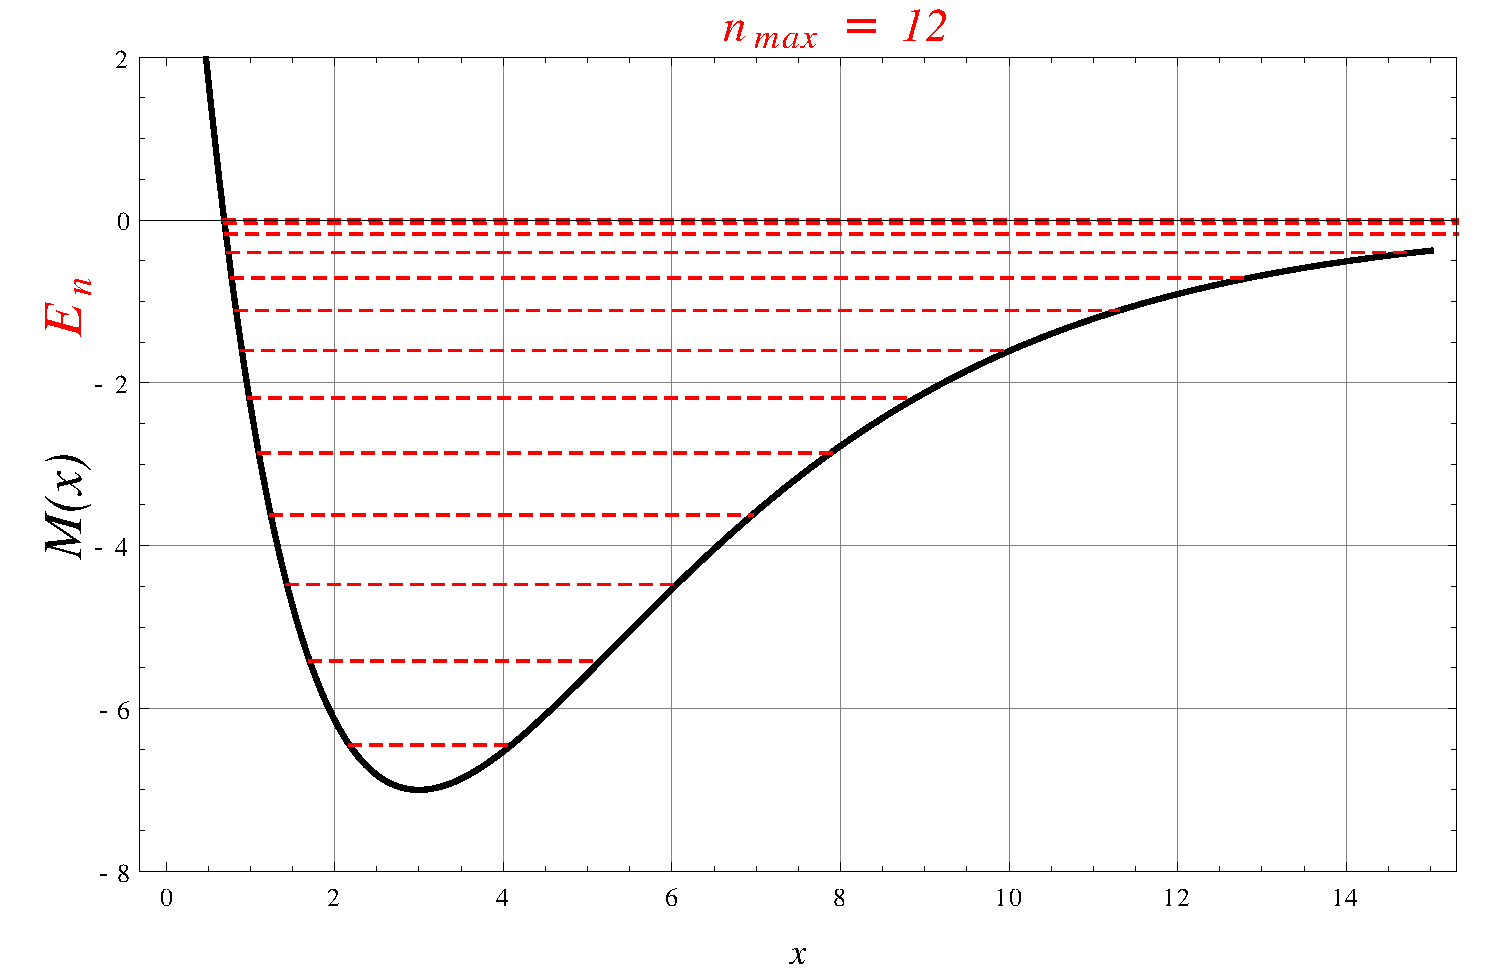
\includegraphics[width=0.5\linewidth]{./figures/MorsePlots/Morse7_03_3.pdf}
    }
    \subfloat[][]{
	\label{fig:MorsePlot7_03_4}
	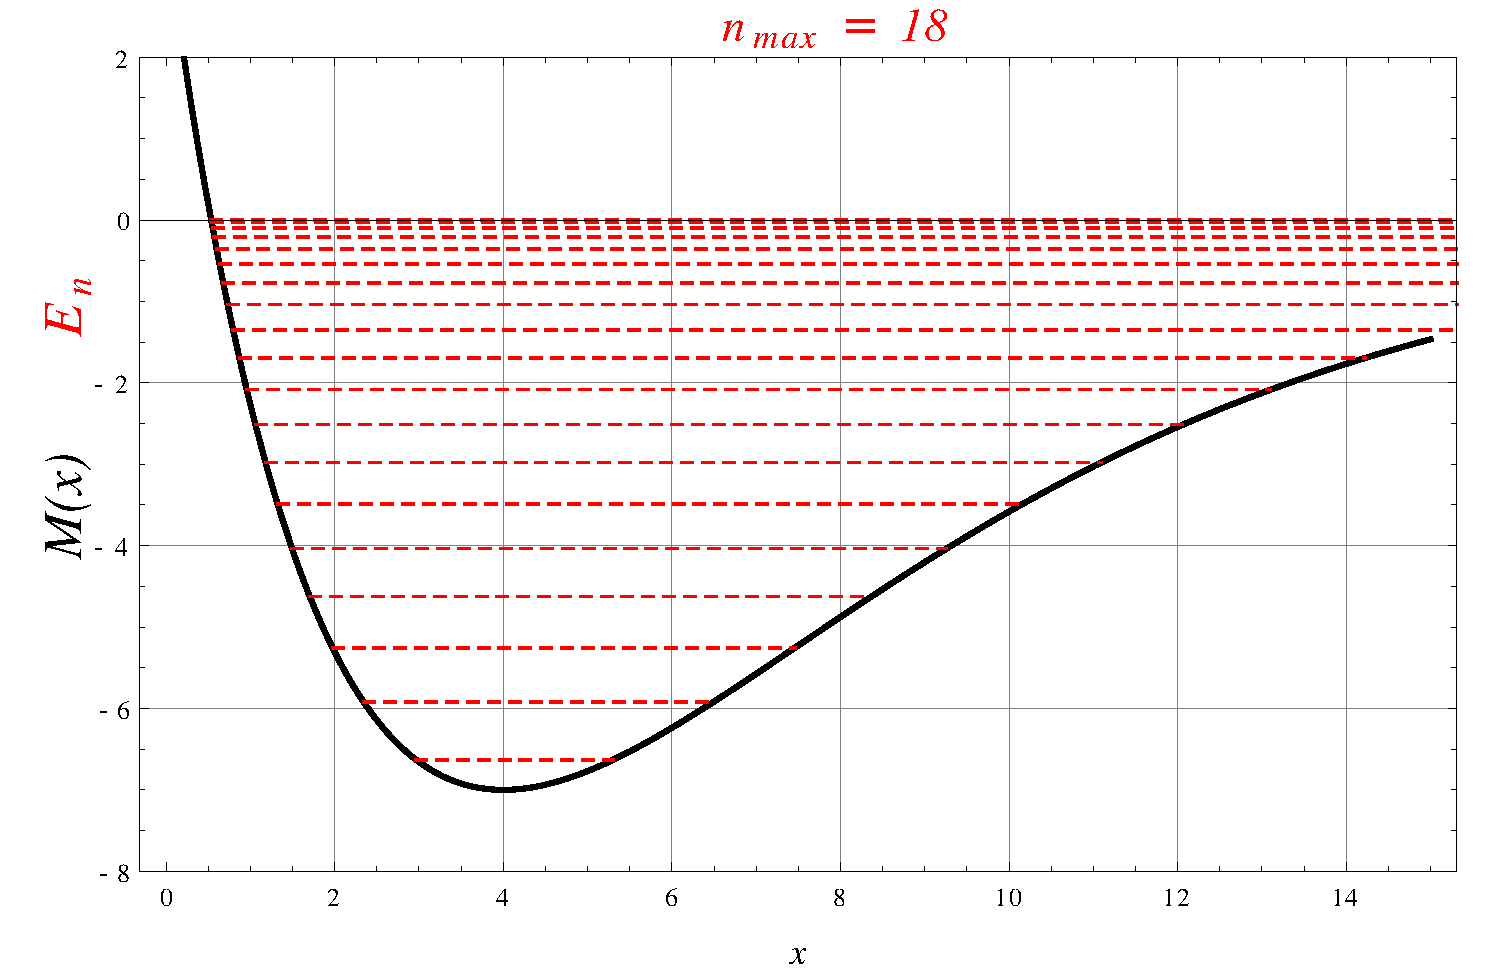
\includegraphics[width=0.5\linewidth]{./figures/MorsePlots/Morse7_02_4.pdf}
    }
    \\

       \caption[Morse potential state energy levels]{Plot of the Morse potential $M(x)$ and the corresponding
    energy levels $E_n$ of bound states for various choices of the parameters $V_0, \beta,$ and $x_0$. At the top
    of each plot we also see the number of bound states for the respective choice of parameters.
    \subref{fig:MorsePlot7_08_3} $V_0=7.0$, $\beta=0.8$ and $x_0=3.0$ ($n_{\text{max}}=4$)
    \subref{fig:MorsePlot5_05_3} $V_0=5.0$, $\beta=0.5$ and $x_0=3.0$ ($n_{\text{max}}=6$)
    \subref{fig:MorsePlot7_03_3} $V_0=7.0$, $\beta=0.3$ and $x_0=3.0$ ($n_{\text{max}}=12$)
    \subref{fig:MorsePlot7_03_4} $V_0=7.0$, $\beta=0.2$ and $x_0=4.0$ ($n_{\text{max}}=18$)
    \label{fig:MorsePlots}
    }

\end{figure}

In Figure \ref{fig:MorsePlots} we can see how the parameters affect width and depth of the potential well. On can also observe
that, in constrast to the harmonic oscillator energy levels, the Morse levels are not equally spaced but get closer together as the energy
approaches zero.\\

As it can be seen in the plots and it will be shown below, the number of discrete bound states
depends on the choice of these parameters, too.
The set of Hagedorn wave packets is a complete orthonormal basis of $L^2(\mathbb{R})$ which theoretically allows for
arbitrary precise approximation. It needs to be investigated whether in the case of Morse wave packets the finite basis leads to good approximations.\\


% section The Morse Potential (end)

\section{Wave packet dynamics} % (fold)
\label{sec:Wave packet dynamics}
In the following we present the time-stepping algorithm for Hagedorn wave packets as proposed by \cite{FGL_semiclassical_dynamics} which can be seen as a template for what we
wish to accomplish in the case of Morse wave packets. The algorithm computes the dynamics of quantum particles for the semi-classical Schrödinger
equation
\begin{equation}
    \label{eq:sctdse}
    i\varepsilon^2\pdiff{\psi}{t}=\mathcal{H}\psi
\end{equation}
with $\varepsilon$ being the scaled Planck constant and  $\psi(x,t)$ with $x,\;t\in\mathbbm{R}$.\\
It is assumed that the Hamiltonian $\mathcal{H}$ can be split as follows into kinetic and Potential part:
\begin{equation}
	\mathcal{H}=T+V,\quad\begin{cases}
	    T&=-\frac{\varepsilon^4}{2}\pdiff{^2}{x^2}, m>0\\
	    V&=V(x)\in\mathbbm{R}
	\end{cases}
\end{equation}
Grid-based methods for solving \eqref{eq:sctdse} usually face highly oscillatory solutions, where wave packets typically have a width
$\sim\varepsilon$ and oscillation wavelengths $\sim \varepsilon^2$. This needs very fine resolutions to achieve the desired accuracy, in particular,
when applied to higher dimensions. On the other hand, the proposed algorithm is essentially grid-free since only the wave packet parameters are evolved
in time using a time-stepping algorithm with splitting into kinetic part, quadratic potential and remainder potential.

\subsection{Hagedorn wave packets} % (fold)
\label{sub:Hagedorn wave packets}
Hagedorn wave packets are basically a product of complex Gaussians and polynomials. Hagedorn \cite{H_ladder_operators} parametrizes such a wave packet as
\begin{equation}
    \label{eq:HG_wavepacket}
    \phi_0[q,p,Q,P](x)=(\pi\varepsilon^2)^{-\frac{N}{4}}(\det Q)^{\frac{1}{2}}\exp\left(\frac{1}{2\varepsilon^2}(x-q)^TPQ^{-1}(x-q)+\frac{i}{\varepsilon^2}p^T(x-q) \right).
\end{equation}
In this formulation $q,p\in\mathbbm{R}$ represent position and momentum of a wave packet while the additional Parameters $P,Q\in\mathbb{C}$ satisfy
\begin{align}
	\label{eq:HG_param_relations}
	\begin{split}
	Q^TP-P^TQ&=0\\
	Q^HP-P^HQ&=2
	\end{split}
\end{align}
and can be interpreted as the width of the wave packet in position and momentum space,
respectively.
% subsection Hagedorn wave packets (end)

\subsection{Ladder operators} % (fold)
\label{sub:Ladder Operators}

% subsection Ladder Operators (end)
In analogy to the operator-algebraic solution of the harmonic oscillator, Hagedorn defines the following raising ($\mathcal{R}$)
and lowering ($\mathcal{L}$) operators:
\begin{align}
    \label{eq:HG_ladder}
    \begin{split}
    \mathcal{R}&=-\frac{i}{\sqrt{2\epsilon}}\left(P^*(x-q)+Q^*(y-p)\right)\\
    \mathcal{L}&=\frac{i}{\sqrt{2\epsilon}}\left(P^T(x-q)+Q^T(y-p)\right)
    \end{split}
\end{align}
where $x$ and $y=-i\epsilon\pdiff{}{x}$ correspond to the position and momentum operator, respectively.\\

Application of these operators on our wave packets yields
\begin{equation}
    \label{eq:HG_ladder_applied}
    \phi_{k+1}=\frac{1}{\sqrt{k+1}}\mathcal{R}\phi_k,\quad \phi_{k-1}=\frac{1}{\sqrt{k}}\mathcal{L}\phi_k.
\end{equation}
Rewriting \eqref{eq:HG_ladder} allows to express the position operator as
\begin{equation}
    x-q=\sqrt{\frac{\epsilon}{2}}(Q\mathcal{R}+\overline{Q}\mathcal{L})
\end{equation}
leading to the important 3-term-recurrence relation
\begin{equation}
    Q\sqrt{k+1}\phi_{k+1}(x)=\sqrt{\frac{2}{\epsilon}}(x-q)\phi_k(x)-\overline{Q}\sqrt{k}\phi_{k-1}(x),
\end{equation}
which allows the numerical computation of the higher states $\phi_k$.\\


\subsection{Diagonalization of Quadratic Hamiltonians} % (fold)
\label{sub:DiagonalizationHGHam}
The most important application of these ladder operators is the exact diagonalization of any classical Hamiltonian of the form
\begin{equation}
    \label{eq:HG_Hamiltonian}
    \mathcal{H}=\frac{1}{2}\left(\alpha p^2+\beta(xp+px)+\gamma x^2\right)
\end{equation}
which can be written as
\begin{equation}
	\label{eq:HG_OpHamiltonian}
	    \mathcal{H}=\frac{\hbar\omega}{2}(\mathcal{R}\mathcal{L}+\mathcal{L}\mathcal{R})\;,
\end{equation}
where
\begin{align*}
	     Q&=\sqrt{\frac{\alpha}{\omega}}e^{i\theta}, &  P&=i\sqrt{\frac{\gamma}{\omega}}e^{-i\theta}\\
	     \theta&=\frac{1}{2}\sin^{-1}\left(\frac{\beta}{\sqrt{\alpha\gamma}}\right),
	     &\omega^2&=(\alpha\gamma^2-\beta^2)\;.
\end{align*}

The eigenvectors of this Hamiltonian are the wave packets $\phi_k(q,p,Q,P)$ together with the corresponding well-known harmonic oscillator
eigenvalues $\hbar\omega(k+\frac{1}{2})$.\\

If we now introduce time-dependence in the quantum mechanical version of the above Hamiltonian \eqref{eq:HG_Hamiltonian} by considering
\begin{equation}
    \label{eq:HG_TimeDepHamiltonian}
    \mathcal{H}(x,p,t)	=-\frac{\alpha(t)\varepsilon^4}{2}\pdiff{^2}{x}
		        -i\frac{\beta(t)\varepsilon^2}{2}\left(x\pdiff{}{x}+\pdiff{}{x}x\right)
			+\frac{\gamma(t)}{2}x^2-i\varepsilon^2\delta(t)\pdiff{}{x}+\epsilon(t)x+\zeta(t)\;,
\end{equation}
we obtain the desired connection between the time evolution of the system and the time evolution of the wave packet parameters:
\begin{align}
    \begin{split}
	\dot{q}(t)&=\beta(t)q(t)+\alpha(t)\eta(t)+\delta(t)\\
	\dot{p}(t)&=-\gamma(t)q(t)-\beta(t)p(t)-\epsilon(t)\\
	\dot{Q}(t)&=\beta(t)Q(t)+\alpha(t)P(t)\\
	\dot{P}(t)&=\gamma(t)Q(t)+\beta(t)P(t)\\
	\dot{S}(t)&=\alpha(t)\frac{\eta^2(t)}{2}-\gamma(t)\frac{\alpha^2(t)}{2}-\epsilon(t)q(t)-\zeta(t)
    \end{split}
\end{align}


Finally, we obtain the following approximation to \eqref{eq:sctdse}:
\begin{equation}
    \label{eq:HG_approx_soln}
    u(x,t)=e^{\frac{iS(t)}{\varepsilon^2}}\sum_{k=0}^{M} c_k(t)
    \phi_k[q(t),p(t),Q(t),P(t)](x).
\end{equation}
The wave packet parameters $q(t), p(t), Q(t), P(t)$ as well as the global phase $S(t)$ and the
expansion coefficients $c_k(t)$, which together form the full parameter set
\begin{equation}
    \label{eq:parameter_set}
    \Pi(t)=\left\lbrace q(t),p(t),Q(t),P(t),S(t)\right\rbrace,\quad c_k(t),
\end{equation}
can then be evolved using a time-stepping algorithm without having to discretize in space.

\subsection{Splitting and Time-stepping} % (fold)
\label{sub:Splitting and Time-stepping}
The Schrödinger equation \eqref{eq:sctdse} is split into a kinetic part (free Schrödinger equation)
\begin{equation}
    \label{eq:tdse_free}
    i\varepsilon^2\pdiff{\psi}{t}=-\frac{\varepsilon^4}{2m}\pdiff{\psi^2}{x^2}
\end{equation}
and a potential part
\begin{equation}
    \label{eq:tdse_pot}
    i\varepsilon^2\pdiff{\psi}{t}=V(x)\psi
\end{equation}
where the later will be again decomposed into a quadratic part $U$ at current position $q$ and the non-quadratic remainder $W$.\\
The free Schrödinger equation \eqref{eq:tdse_free} and, according to Theorem 2.5 in \cite{H_ladder_operators}, the quadratic potential part
\eqref{eq:tdse_pot} can be solved exactly with the wave function remaining in the Hagedorn form, whereas for the remainder potential one has to
rely on a Galerkin approximation.

% subsection Splitting and Time-stepping (end)



% section Wave packet dynamics (end)

\end{chapter}
